\chapter{Dataset}
\label{sec:Chapter3}
Dataset pro tuto práci je vygenerován synteticky, pozadí jsou focena kamerou StereoLabs ZED 2 a popředí synteticky vykresleným modelem auta LEGO Hot Rod 42022. Pro tvorbu syntetického datasetu, augmentaci dat a transformaci augmentovaných pozic klíčových bodů/ohraničujících boxů byla využita knihovna \texttt{albumenations} v rámci jazyka Python 3. 

V rámci několika světelných nastavení bylo nafoceno v auto-kalibračním režimu kamery pozadí pro generování dat ve formátu PNG s následujícími parametry: \texttt{1920$\times$1080, 8-bit/color RGB, non-interlaced}. Nutno podotknout, že při reálném použití by v daný moment platné parametry kamery sloužily ke generování dvou vstupů do funkce \texttt{solvePnP}, a to matice kamery a parametru \texttt{distCoeffs} do funkce:
\begin{itemize}
    \item Ohnisková vzdálenost -- $f_x$, $f_y$
    \item Hlavní body -- $c_x$, $c_y$
    \item Zkreslení objektivu -- $k_1$, $k_2$, $k_3$, $p_1$, $p_2$
\end{itemize}

Objektem zájmu v této práci je 3D model LEGO automobilu, který je identický vůči tomu použitému v předchozí bakalářské práci \cite{mojebp}. Zde je dostupná sada syntetických renderovaných snímků celého modelu v různých natočeních kamery soustředěné na střed objektu. Sada obsahuje identické snímky v 5 různých virtuálních nastaveních, každé s odlišnými světelnými podmínkami. Součástí modelu jsou také pozice klíčových bodů v lokálním souřadném systému společně s jejich normálami. Každý snímek vykresleného modelu má taky v páru se sebou uložen \texttt{NumPy}/\texttt{pickle} slovník s následujícími metadaty:
\begin{itemize}
    \item MV matice
    \item MVP matice
    \item Pozice kamery v kartézském souřadném systému
\end{itemize}
Normály společně s těmito metadaty nám v tomto kontextu mohou posloužit jako praktický indikátor viditelnosti.


\begin{figure}[ht]
\centering

% width is 0.86in corresponding to 150DPI for 128/128
\newcommand{\subfiguresize}{.15\textwidth}
\newcommand{\imagewidth}{2.1in}
\newcommand{\hspacesize}{.1in}

% Example of using minipage for an image block
\newcommand{\insertimage}[1]{%
  \begin{minipage}{\imagewidth}
    \centering
    \includegraphics[width=\imagewidth]{#1}
  \end{minipage}
}

% Row 1
\subfloat[EA408]{%
  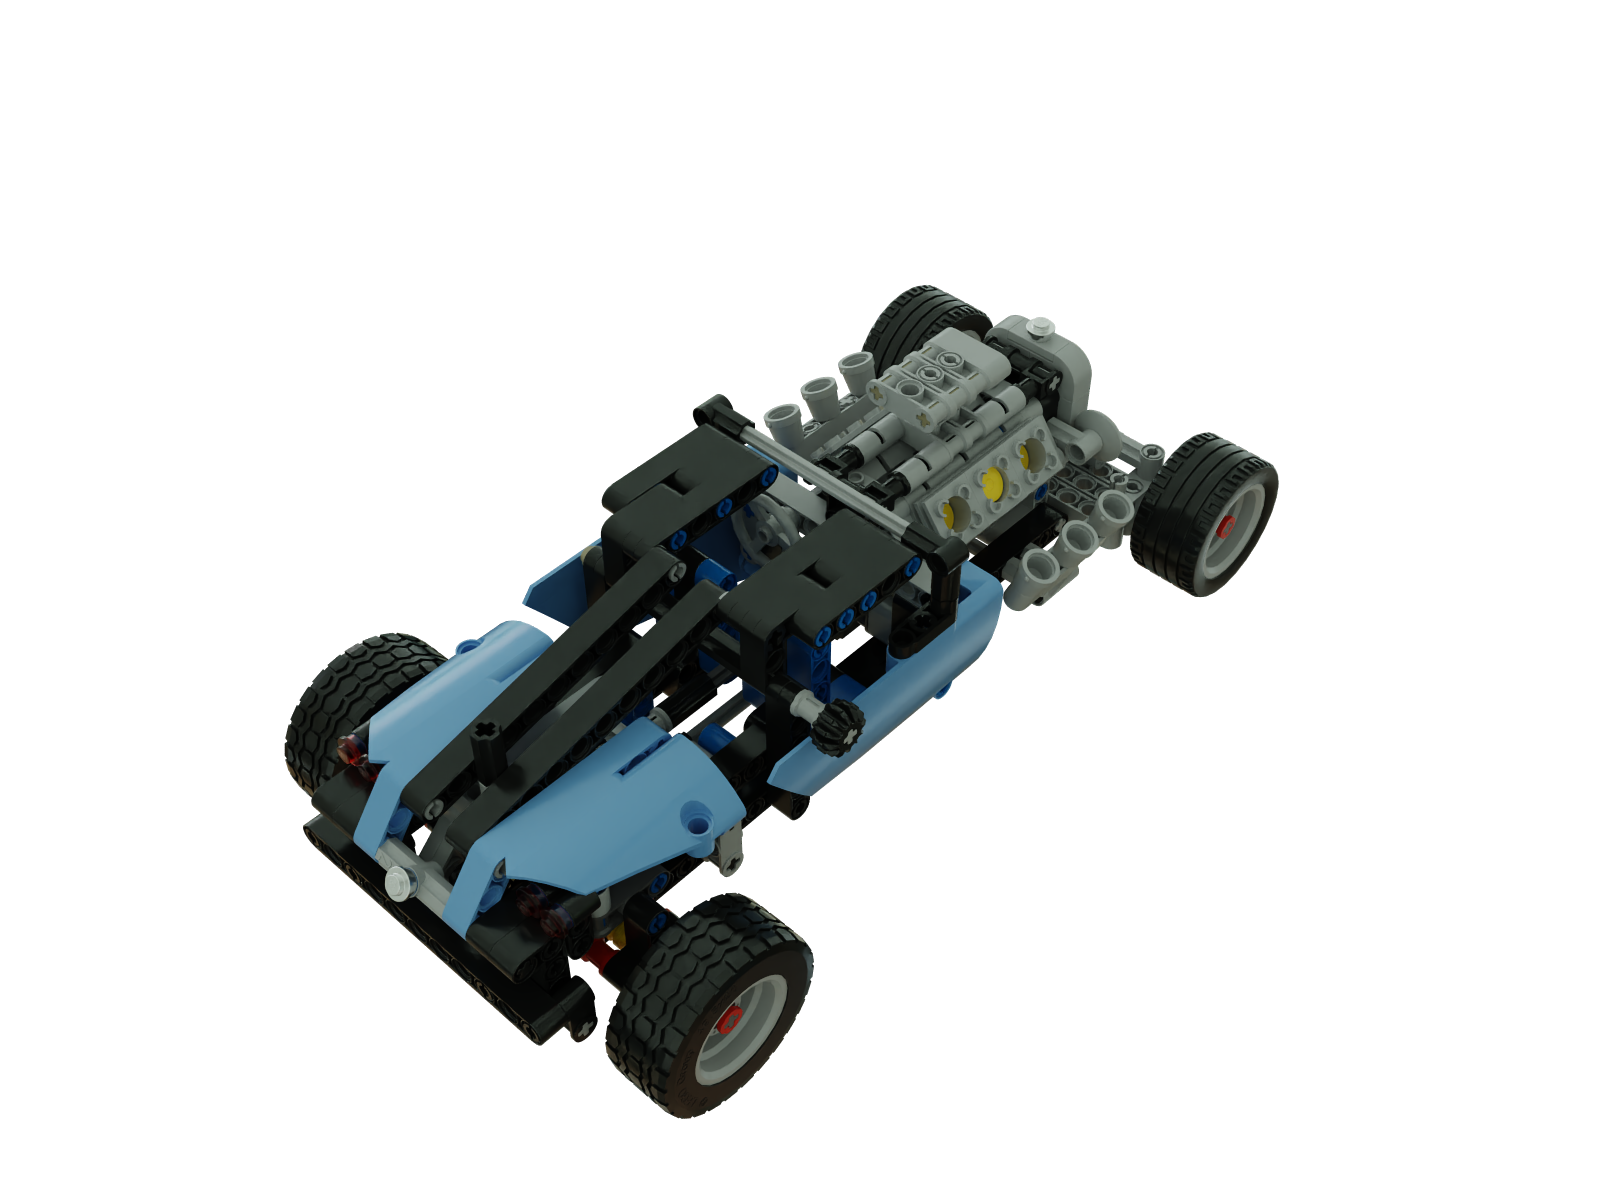
\includegraphics[width=\imagewidth]{Figures/ea408.png}%
  \label{fig:sp00}%
}\hspace{\hspacesize}%
\subfloat[EA408 světlé]{%
  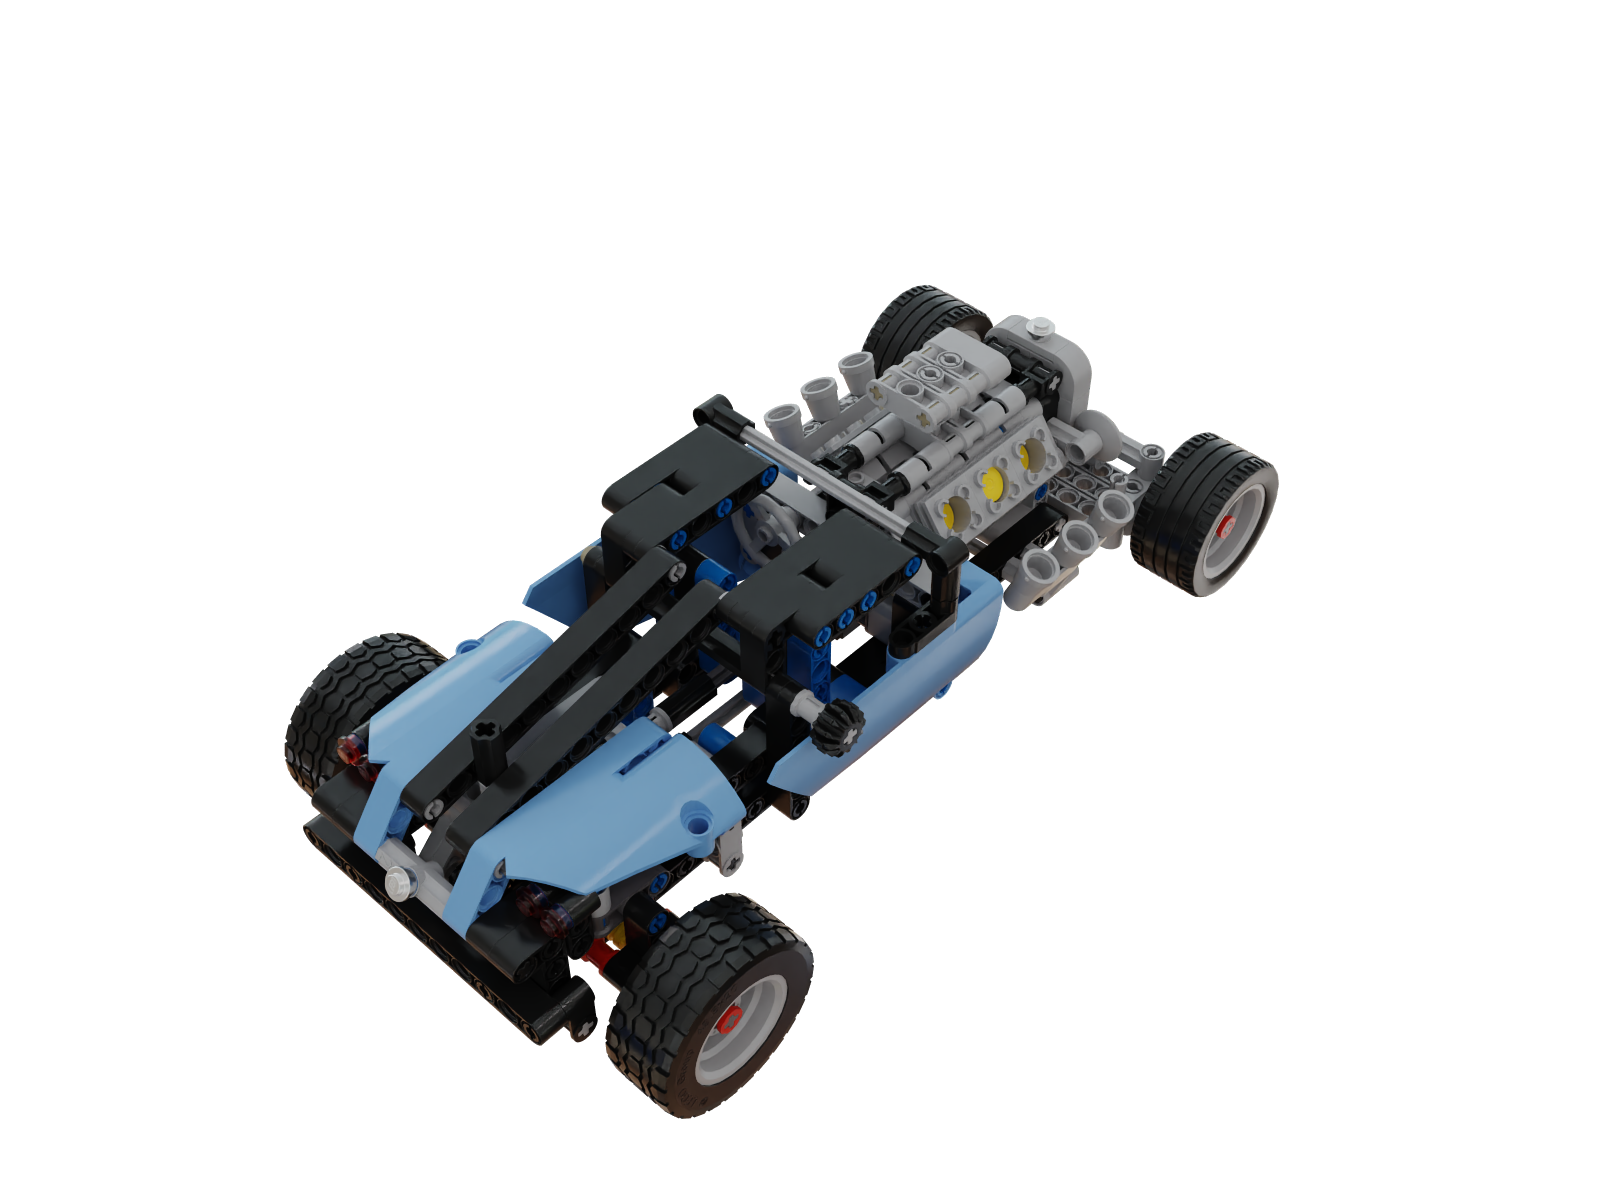
\includegraphics[width=\imagewidth]{Figures/ea408_light.png}%
  \label{fig:sp01}%
}\hspace{\hspacesize}%
\subfloat[Scéna typu \texttt{empty\_warehouse}]{%
  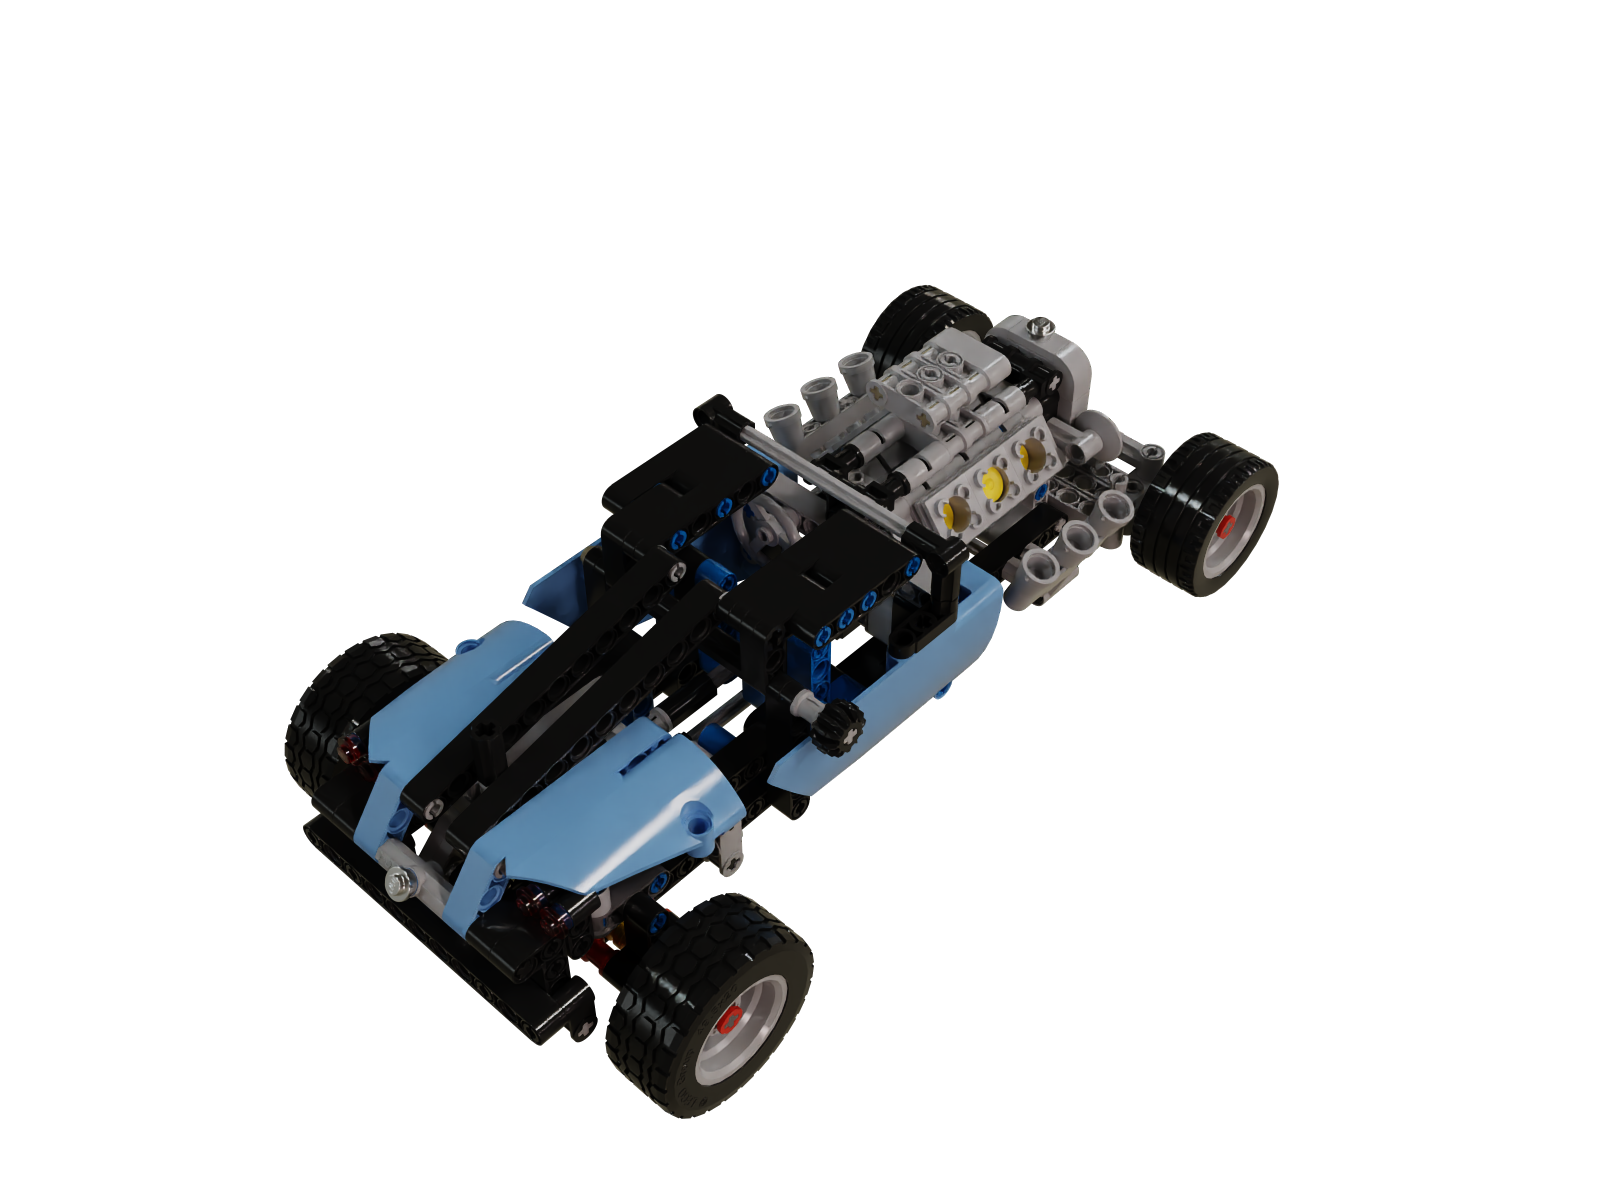
\includegraphics[width=\imagewidth]{Figures/empty_warehouse.png}%
  \label{fig:sp02}%
}

% Row 2
\subfloat[Scéna typu \texttt{lebombo}]{%
  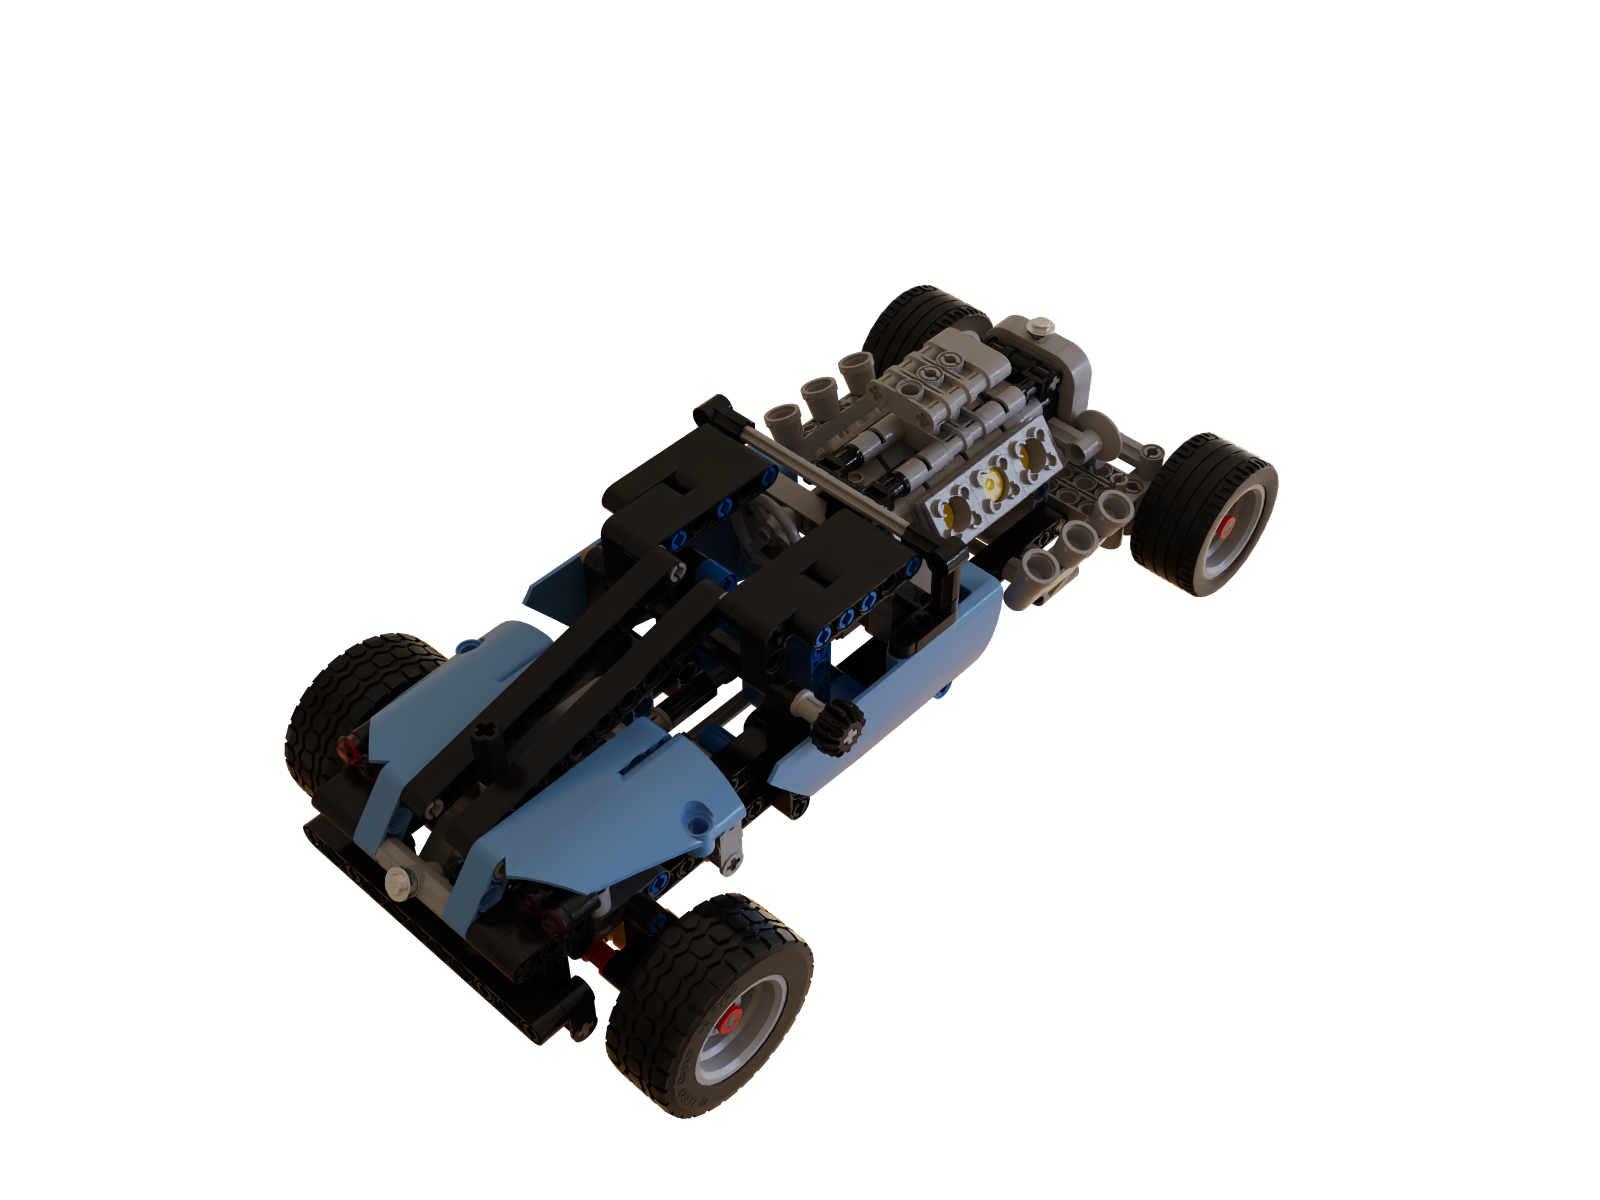
\includegraphics[width=\imagewidth]{Figures/lebombo.png}%
  \label{fig:sp09}%
}\hspace{\hspacesize}%
\subfloat[Scéna typu \texttt{lilienstein}]{%
  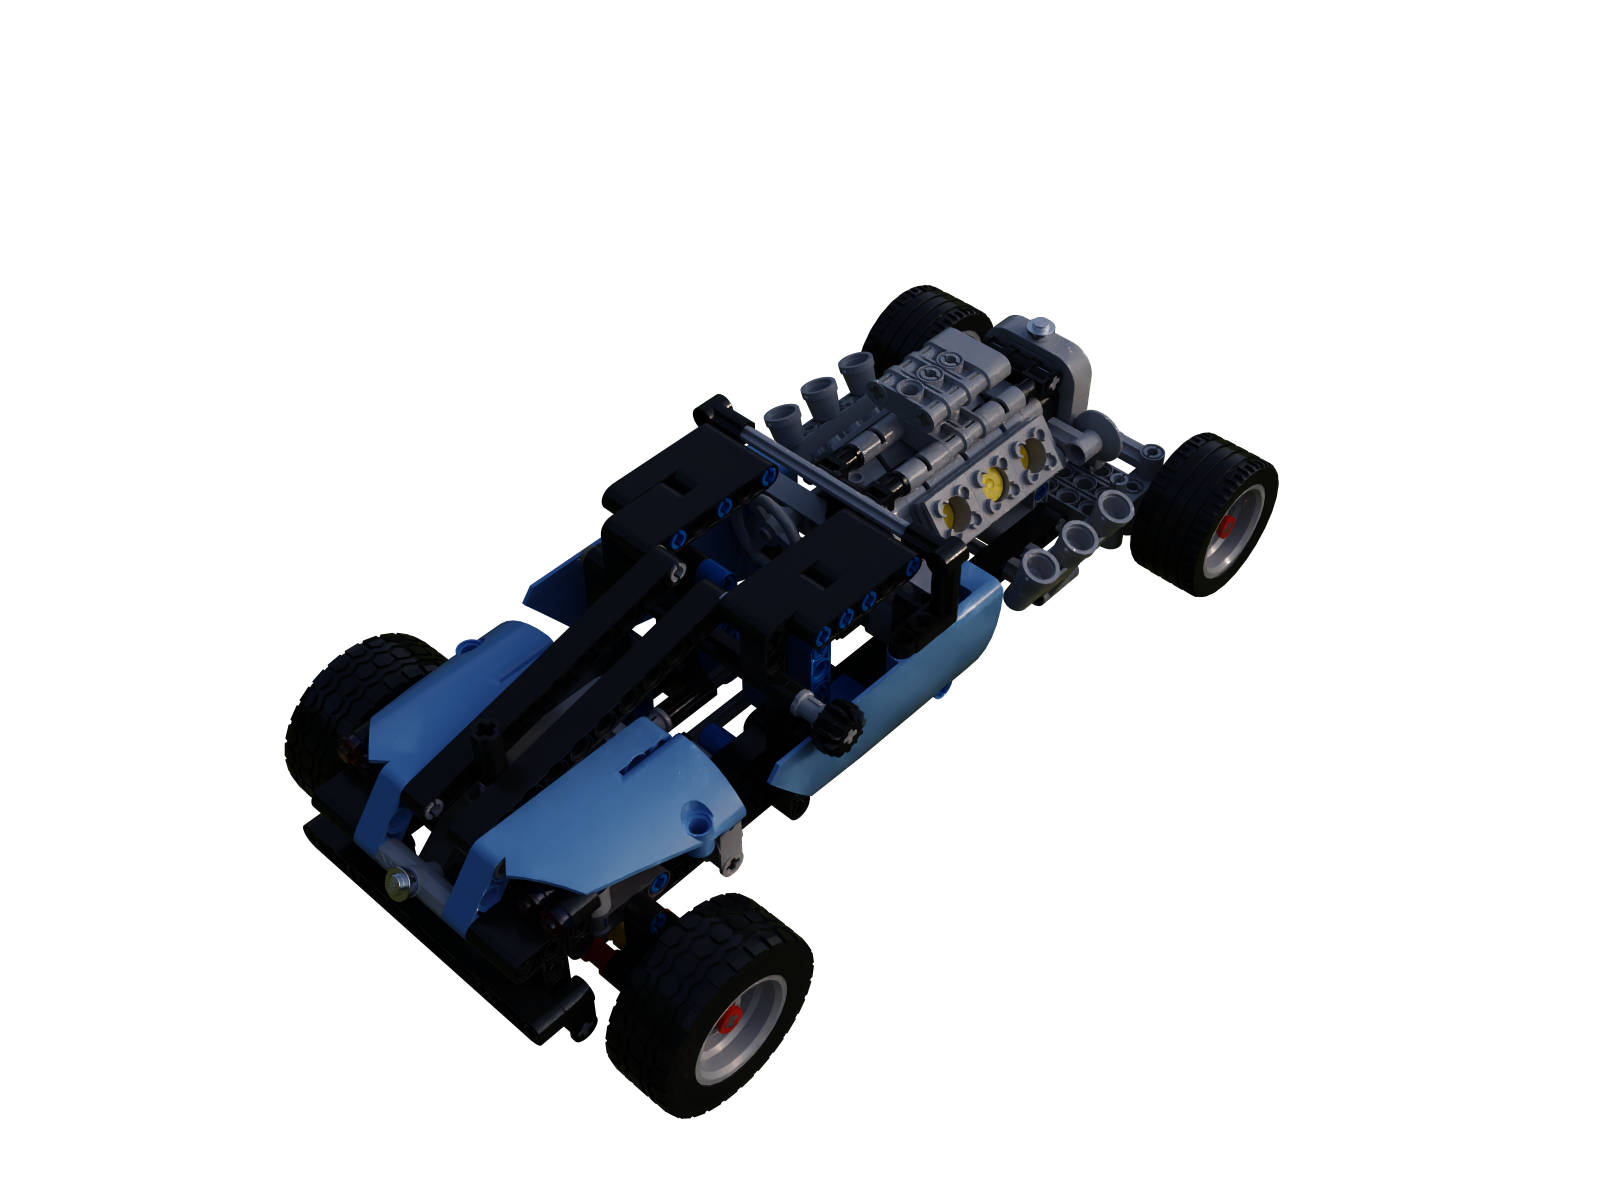
\includegraphics[width=\imagewidth]{Figures/lilienstein.png}%
  \label{fig:sp10}%
}\hspace{\hspacesize}%
\subfloat{%
  \hspace{\imagewidth}
}

\caption[Příklady syntetických snímků z datasetu]{Příklady syntetických snímků z datasetu}
\label{fig:synthetic_images}
\end{figure}


\begin{figure}[hb]
\centering
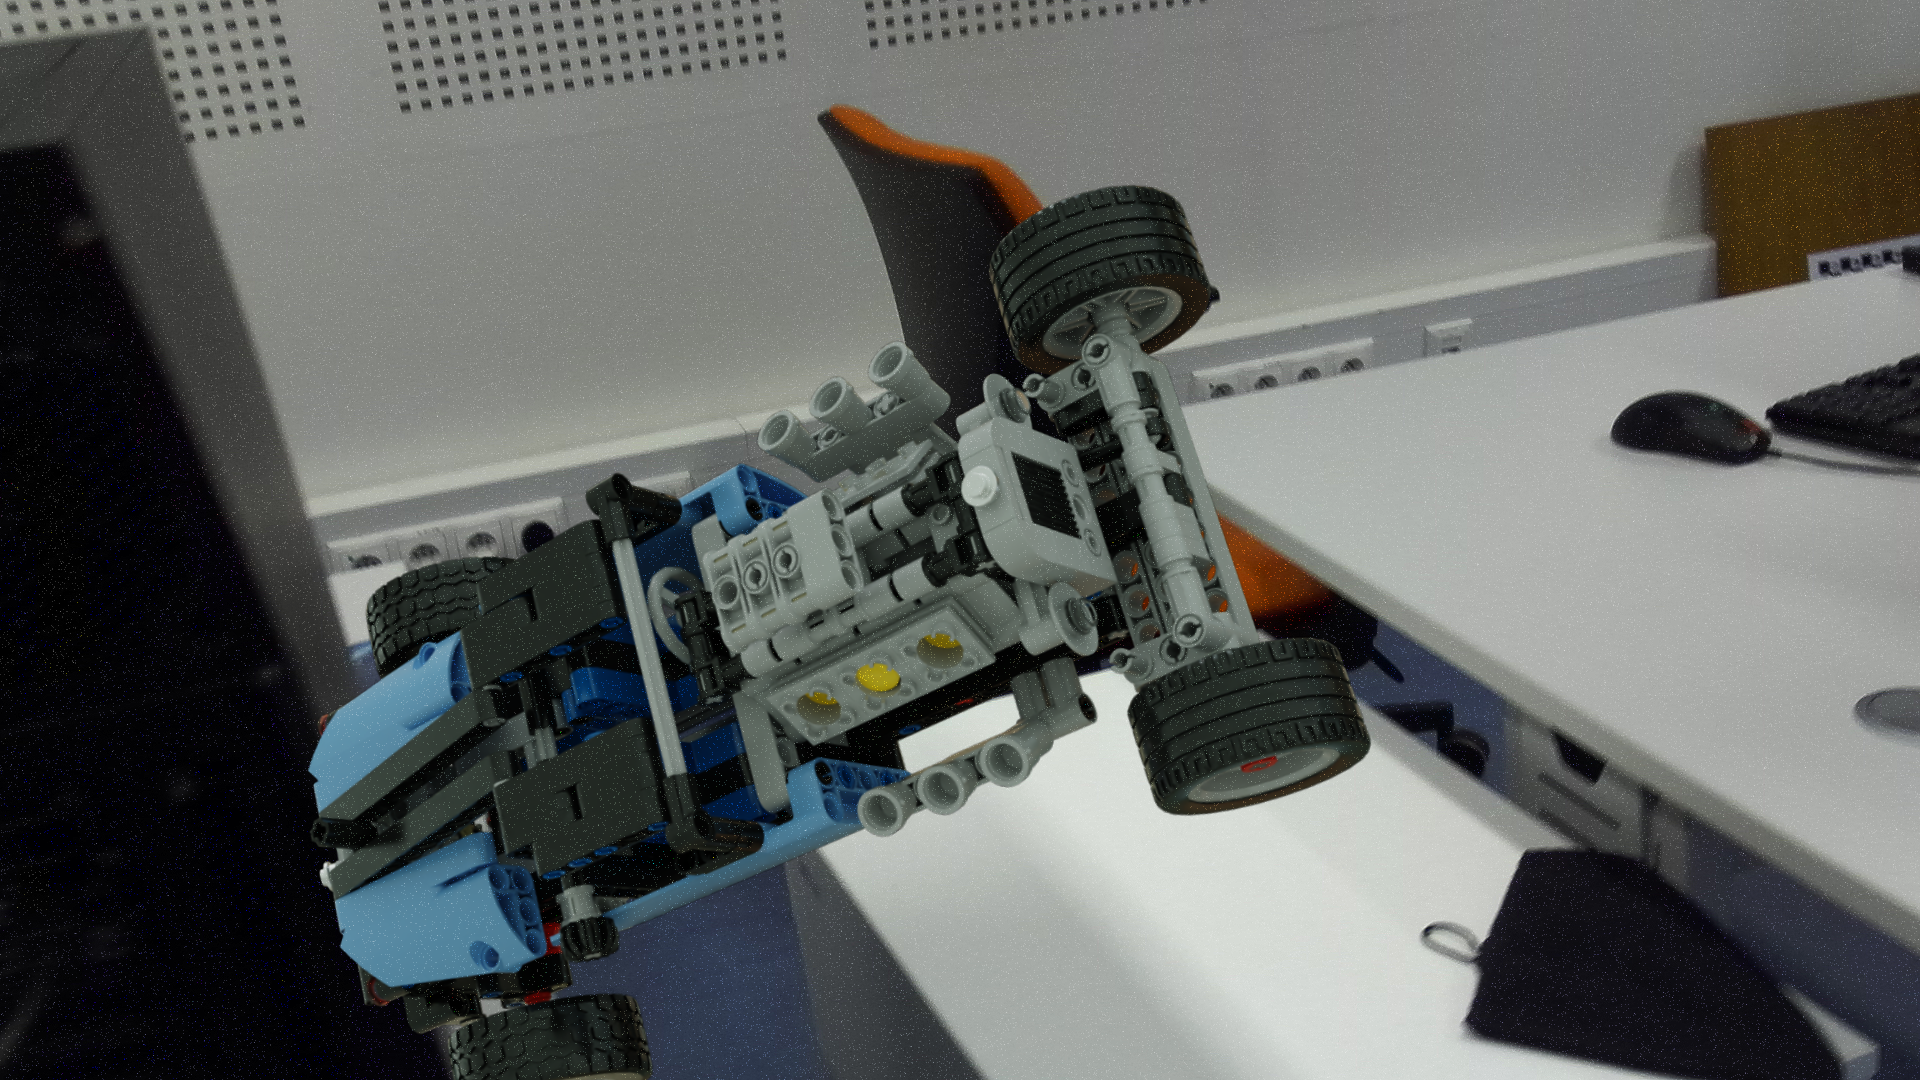
\includegraphics[width=0.4\textwidth,keepaspectratio]{Figures/train_EA408_199.png}
\caption{Příklad snímku ze syntetického datasetu}
\label{fig:trainimg}
\end{figure}